% last synchronized to 'dbc28949bf4332ac86d84b95705fbea9af4f84f7'
\chapter{The Ethernet Model}
\label{cha:ethernet}

% TODO: comment numWirelessPorts in MacRelayUnitPP
% TODO: comment origByteLength in EtherFrame
% FIXME: wrong header length in EtherFrame.msg

\section{Overview}

Variations: 10Mb/s ethernet, fast ethernet, Gigabit Ethernet, Fast Gigabit Ethernet, full duplex

The Ethernet model contains a MAC model (\nedtype{EtherMAC}), LLC model (\nedtype{EtherLLC}) as well
as a bus (\nedtype{EtherBus}, for modelling coaxial cable) and a hub (\nedtype{EtherHub}) model.
A switch model (\nedtype{EtherSwitch}) is also provided.

\begin{itemize}
  \item \nedtype{EtherHost} is a sample node with an Ethernet NIC;
  \item \nedtype{EtherSwitch}, \nedtype{EtherBus}, \nedtype{EtherHub} model switching hub, repeating hub and
        the old coxial cable;
  \item basic compnents of the model: \nedtype{EtherMAC}, \nedtype{EtherLLC}/\nedtype{EtherEncap} module types,
        \nedtype{MACRelayUnit} (\nedtype{MACRelayUnitNP} and \nedtype{MACRelayUnitPP}), \nedtype{EtherFrame} message type,
        \cppclass{MACAddress} class
\end{itemize}

Sample simulations:

\begin{itemize}
  \item the \nedtype{MixedLAN} model contains hosts, switch, hub and bus
  \item the \nedtype{LargeNet} model contains hundreds of computers, switches and hubs
        (numbers depend on model configuration in largenet.ini) and mixes all
        kinds of Ethernet technologies
\end{itemize}

\subsection{Implemented Standards}

The Ethernet model operates according to the following standards:

\begin{itemize}
  \item Ethernet: IEEE 802.3-1998
  \item Fast Ethernet: IEEE 802.3u-1995
  \item Full-Duplex Ethernet with Flow Control: IEEE 802.3x-1997
  \item Gigabit Ethernet: IEEE 802.3z-1998
\end{itemize}

\section{Physical layer}

The nodes of the Ethernet networks are connected by coaxial,
twisted pair or fibre cables. There are several cable types specified
in the standard.

In the INET framework, the cables are represented by connections.
The connections used in Ethernet LANs must be derived from
\nedtype{DatarateConnection} and should have their \fpar{delay} and
\fpar{datarate} parameters set.
The delay parameter can be used to model the distance between the
nodes. The datarate parameter can have four values:

\begin{itemize}
  \item \ttt{10Mbps} classic Ethernet
  \item \ttt{100Mbps} Fast Ethernet
  \item \ttt{1Gbps} Gigabit Ethernet
  \item \ttt{10Gbps} Fast Gigabit Ethernet
\end{itemize}


\subsection{EtherBus}

The \nedtype{EtherBus} component can model a common coaxial cable
found in earlier Ethernet LANs. The nodes are attached at specific
positions of the cable. If a node sends a packet, it is transmitted
in both direction by a given propagation speed.

The gates of the \nedtype{EtherBus} represent taps. The positions
of the taps are given by the \fpar{positions} parameter as a
space separated list of distances in metres. If there are more
gates then positions given, the last distance is repeated.
The bus component send the incoming message in one direction and
a copy of the message to the other direction (except at the ends).
The propagation delays are computed from the distances of the taps
and the \fpar{propagationSpeed} parameter.

Messages are not interpreted by the bus model in any way, thus the bus
model is not specific to Ethernet in any way. Messages may
represent anything, from the beginning of a frame transmission to
end (or abortion) of transmission.

% FIXME #356 NED comment is wrong: data rate must not be zero!
% FIXME #354 default propagation speed is wrong (should be 2e8mps)
%            btw there is a hard coded propagation speed in EtherMACBase.cc

\subsection{EtherHub}

Ethernet hubs are a simple broadcast devices. Messages arriving on a port
are regenerated and broadcast to every other port.

The connections connected to the hub must have the same data rate.
Cable lengths should be reflected in the delays of the connections.

Messages are not interpreted by the \nedtype{EtherType} hub model in any way,
thus the hub model is not specific to Ethernet. Messages may
represent anything, from the beginning of a frame transmission to
end (or abortion) of transmission.

The hub module collects the following statistics:

\begin{itemize}
\item \ttt{pkBytes} handled packets length (vector)
\item \ttt{messages/sec} number of packets per seconds (scalar)
\end{itemize}

% FIXME #356 NED comment is wrong: data rate must not be zero!
% TODO: model delay in hubs: class I device 140 bit time, class II device 92 bit time (for fast ethernet)

\section{MAC layer}

The Ethernet MAC (Media Access Control) layer transmits the Ethernet frames on
the physical media. This is a sublayer within the data link layer. Because
encapsulation/decapsulation is not always needed (e.g. switches does not do
encapsulation/decapsulation), it is implemented in a separate modules
(\nedtype{EtherEncap} and \nedtype{EtherLLC}) that are part of the LLC layer.

\begin{center}
\setlength{\unitlength}{1mm}
\begin{picture}(50,50)
\put(2,47){Network layer}
\put(12,35){\vector(0,1){10}}
\put(12,45){\vector(0,-1){10}}
\put(0,15){\line(1,0){50}}
\put(50,15){\line(0,1){20}}
\put(50,35){\line(-1,0){50}}
\put(0,35){\line(0,-1){20}}
\put(25,25){\line(0,1){10}}
\put(0,25){\line(1,0){50}}
\put(10,28){LLC}
\put(27,28){MAC Relay}
\put(22,18){MAC}
\put(25,5){\vector(0,1){10}}
\put(25,15){\vector(0,-1){10}}
\put(15,2){Physical layer}
\end{picture}
\end{center}

Nowadays almost all Ethernet networks operate using full-duplex
point-to-point connections between hosts and switches. This means
that there are no collisions, and the behaviour of the MAC component
is much simpler than in classic Ethernet that used coaxial cables and
hubs. The INET framework contains two MAC modules for Ethernet:
the \nedtype{EtherMACFullDuplex} is simpler to understand and easier to extend,
because it supports only full-duplex connections. The \nedtype{EtherMAC}
module implements the full MAC functionality including CSMA/CD, it
can operate both half-duplex and full-duplex mode.

\subsection*{Packets and frames}

The environment of the MAC modules is described by the \nedtype{IEtherMAC}
module interface. Each MAC modules has gates to connect to the physical
layer (\ttt{phys\$i} and \ttt{phys\$o}) and to connect to the upper layer
(LLC module is hosts, relay units in switches): \ttt{upperLayerIn} and
\ttt{upperLayerOut}.

When a frame is received from the higher layers, it must be an
\msgtype{EtherFrame}, and with all protocol fields filled out
(including the destination MAC address). The source address, if left empty,
will be filled in with the configured \fpar{address} of the MAC.
% TODO document auto MAC address


Packets received from the network are \msgtype{EtherTraffic} objects.
They are messages representing inter-frame gaps (\msgtype{EtherPadding}),
jam signals (\msgtype{EtherJam}), control frames (\msgtype{EtherPauseFrame})
or data frames (all derived from \msgtype{EtherFrame}). Data frames
are passed up to the higher layers without modification.
In \fpar{promiscuous} mode, the MAC passes up all received frames;
otherwise, only the frames with matching MAC addresses and
the broadcast frames are passed up.

Also, the module properly responds to PAUSE frames, but never sends them
by itself -- however, it transmits PAUSE frames received from upper layers.
See section~\ref{subsec:pause_handling} for more info.

\subsection*{Queueing}

When the transmission line is busy, messages received from the upper layer
needs to be queued.

In routers, MAC relies on an external queue module (see \nedtype{OutputQueue}),
and requests packets from this external queue one-by-one. The name of the
external queue must be given as the \fpar{queueModule} parameer.
There are implementations of \nedtype{OutputQueue} to model finite buffer,
QoS and/or RED.

In hosts, no such queue is used, so MAC contains an internal
queue named \fvar{txQueue} to queue up packets waiting for transmission.
Conceptually, \fvar{txQueue} is of infinite size, but for better diagnostics
one can specify a hard limit in the \fpar{txQueueLimit} parameter -- if this is
exceeded, the simulation stops with an error.

\subsection*{PAUSE handling}
\label{subsec:pause_handling}

The 802.3x standard supports PAUSE frames as a means of flow
control. The frame contains a timer value, expressed as a multiple
of 512 bit-times, that specifies how long the transmitter should
remain quiet. If the receiver becomes uncongested before the
transmitter's pause timer expires, the receiver may elect to send
another PAUSE frame to the transmitter with a timer value of zero,
allowing the transmitter to resume immediately.

\nedtype{EtherMAC} will properly respond to PAUSE frames it receives
(\msgtype{EtherPauseFrame} class),
however it will never send a PAUSE frame by itself. (For one thing,
it doesn't have an input buffer that can overflow.)

\nedtype{EtherMAC}, however, transmits PAUSE frames received by higher layers,
and \nedtype{EtherLLC} can be instructed by a command to send a PAUSE frame to MAC.

% FIXME PAUSE frames should only be sent on full-duplex ethernet.
%       If a switch uses half-duplex mode to connect to hosts, it can ask sending hosts
%       to slow down their sending rates:
%       - force collisions with incoming frames
%       - make it appear as if the channel is busy
% FIXME PAUSE frames should have 0x8808 in the etherType field

\subsection*{Error handling}

If the MAC is not connected to the network ("cable unplugged"), it will
start up in "disabled" mode. A disabled MAC simply discards any messages
it receives. It is currently not supported to dynamically connect/disconnect
a MAC.

CRC checks are modeled by the \fvar{bitError} flag of the packets. Erronous
packets are dropped by the MAC.

\subsection*{Signals and statistics}

Both MAC modules emits the following signals:
\begin{itemize}
  \item \fsignal{txPk} after successful data frame transmission, the data frame
  \item \fsignal{rxPkOk} after successful data frame reception, the data frame
  \item \fsignal{txPausePkUnits} after PAUSE frame sent, the pause time
  \item \fsignal{rxPausePkUnits} after PAUSE frame received, the pause time
  \item \fsignal{rxPkFromHL} when a data frame received from higher layer,
         the data frame
  \item \fsignal{dropPkNotForUs} when a data frame received not addressed
         to the MAC, the data frame
  \item \fsignal{dropPkBitError} when a frame received with bit error, the frame
  \item \fsignal{dropPkIfaceDown} when a message received and the MAC is not connected,
        the dropped message
  \item \fsignal{packetSentToLower} before starting to send a packet on phys\$o gate,
        the packet
  \item \fsignal{packetReceivedFromLower} after a packet received on phys\$i gate,
        the packet (excluding PAUSE and JAM messages and dropped data frames)
  \item \fsignal{packetSentToUpper} before sending a packet on upperLayerOut, the packet
  \item \fsignal{packetReceivedFromUpper} after a packet received on upperLayerIn,
        the packet
\end{itemize}

% FIXME rxPkOkSignal == packetSentToUpperSignal

Apart from statistics can be generated from the signals, the modules collects
the following scalars:

\begin{itemize}
  \item \ttt{simulated time} total simulation time
  \item \ttt{full duplex} boolean value, indicating whether the module operated
          in full-duplex mode
  \item \ttt{frames/sec sent} data frames sent (not including PAUSE frames) per second
  \item \ttt{frames/sec rcvd} data frames received (not including PAUSE frames) per second
  \item \ttt{bits/sec sent}
  \item \ttt{bits/sec rcvd}
\end{itemize}

Note that four of these scalars could be recorded as the count and value of the \fsignal{txPkBytesSignal}
and \fsignal{rxPkBytesSignal} signals resp.

\subsection*{Visual effects}

In the graphical environment, some animation effects help to follow the simulation.
The color of the transmission channel is changed to yellow during transmission, and
turns to red when collision detected. The icon of disconnected MAC modules are grayed out.

The icon of the Ethernet NICs are also colored according to the state of MAC module:
yellow if transmitting, blue if receiving, red if collision detected, white in backoff
and gray in paused state.

%\subsection*{Auto-Negotiation}
% Ethernet Auto-Negotiation not supported



\subsection{EtherMACFullDuplex}

From the two MAC implementation \nedtype{EtherMACFullDuplex} is the simpler one,
it operates only in full-duplex mode (its \fpar{duplexEnabled} parameter fixed to
\ttt{true} in its NED definition). This module does not need to implement
CSMA/CD, so there is no collision detection, retransmission with exponential backoff,
carrier extension and frame bursting. Flow control works as described in section
\ref{subsec:pause_handling}.

% FIXME remove frameBursting from NED def, or fix it to false
%       currently setting it to 'true' has no effect

In the \nedtype{EtherMACFullDuplex} module,
packets arrived at the \ttt{phys\$i} gate are handled when their last bit received.

Outgoing packets are transmitted according to the following state diagram:

\begin{center}
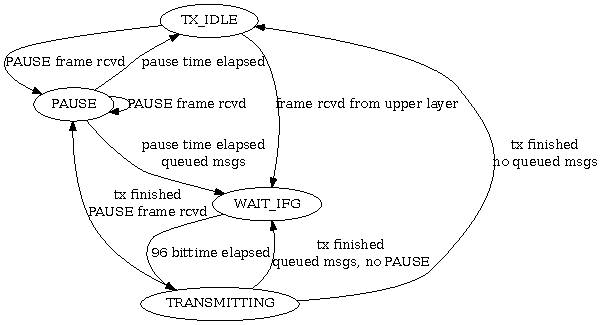
\includegraphics{figures/EtherMACFullDuplex_txstates}
\end{center}

The \nedtype{EtherMACFullDuplex} module records two scalars in addition to the
ones mentioned earlier:
\begin{itemize}
\item \ttt{rx channel idle (\%)}: reception channel idle time
        as a percentage of the total simulation time
\item \ttt{rx channel utilization (\%)}: total reception
        time as a percentage of the total simulation time
\end{itemize}

\subsection{EtherMAC}

Ethernet MAC layer implementing CSMA/CD. It supports both half-duplex and full-duplex operations;
in full-duplex mode it behaves as \nedtype{EtherMACFullDuplex}. In half-duplex  mode
it detects collisions, sends jam messages and retransmit frames upon collisions using
the exponential backoff algorithm. In Gigabit Ethernet networks it supports carrier
extension and frame bursting. Carrier extension can be turned off by setting the
\fpar{carrierExtension} parameter to \ttt{false}.

Unlike \nedtype{EtherMACFullDuplex}, this MAC module processes the incoming packets when their
first bit is received. The end of the reception is calculated by the MAC and
detected by scheduling a self message.

When frames collide the transmission is aborted -- in this case the transmitting
station transmits a jam signal. Jam signals are represented
by a \msgtype{EtherJam} message. The jam message contains the tree identifier
of the frame whose transmission is aborted. When the \nedtype{EtherMAC} receives a jam
signal, it knows that the corresponding transmission ended in jamming and have
been aborted. Thus when it receives as many jams as collided frames, it can
be sure that the channel is free again. (Receiving a jam message marks the
beginning of the jam signal, so actually has to wait for the duration of the jamming.)

The operation of the MAC module can be schematized by the following state chart:

\begin{center}
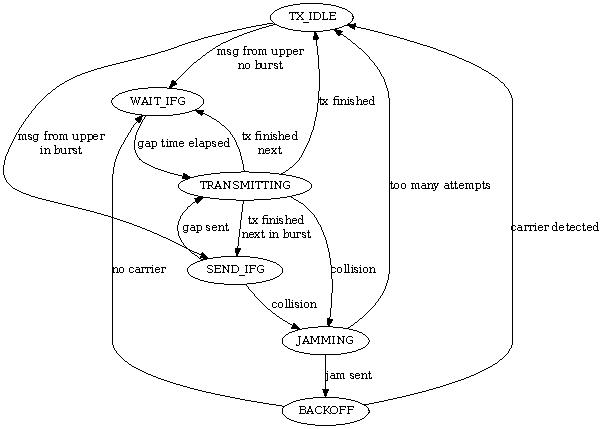
\includegraphics{figures/EtherMAC_txstates}
\end{center}

The module generates these extra signals:
\begin{itemize}
\item \fsignal{collision} when collision starts (received a frame,
         while transmitting or receiving another one; or start to transmit while receiving a frame),
         the constant value 1
\item \fsignal{backoff} when jamming period ended and before waiting according to the
         exponential backoff algorith, the constant value 1
\end{itemize}

These scalar statistics are generated about the state of the line:
\begin{itemize}
  \item \ttt{rx channel idle (\%)} reception channel idle time (full duplex) or channel
         idle time (half-duplex), as a percentage of the total simulation time
  \item \ttt{rx channel utilization (\%)} total successful reception time (full-duplex) or total
         successful reception/transmission time (half duplex), as a percentage
         of the total simulation time
  \item \ttt{rx channel collision (\%)} total unsuccessful reception time, as a percentage
         of the total simulation time
  \item \ttt{collisions} total number collisions (same as count of \fsignal{collisionSignal})
  \item \ttt{backoffs} total number of backoffs (same as count of \fsignal{backoffSignal})
\end{itemize}

% document error conditions (causing error() calls in the code)

% FIXME handleRestransmission() comment is not true: // no beginSendFrames(), because end of jam signal sending will trigger it automatically
%       in case of inner queue, the queued msg is not transmitted
% FIXME should not enter PAUSE state when !duplexMode


\section{Switches}

Ethernet switches play an important role in modern Ethernet LANs. Unlike
passive hubs and repeaters, that work in the physical layer, the switches
operate in the data link layer and routes data frames between the connected
subnets.

While a hub repeats the data frames on each connected line, possibly causing
collisions, switches help to segment the network to small collision domains.
In modern Gigabit LANs each node is connected to the switch direclty
by full-duplex lines, so no collisions are possible. In this case the
CSMA/CD is not needed and the channel utilization can be high.

\subsection{MAC relay units}

INET framework ethernet switches are built from \nedtype{IMACRelayUnit}
components. Each relay unit has N input and output gates for sending/receiving
Ethernet frames. They should be connected to \nedtype{IEtherMAC} modules.

Internally the relay unit holds a table for the destination address -> output
port mapping. When it receives a data frame it updates the table with the
source address->input port. The table can also be pre-loaded from a text file
while initializing the relay unit. The file name given as the \fpar{addressTableFile}
parameter. Each line of the file contains a hexadecimal MAC address and a decimal port
number separated by tabs. Comment lines beginning with '\#' are also allowed:

\begin{verbatim}
01 ff ff ff ff    0
00-ff-ff-ee-d1    1
0A:AA:BC:DE:FF    2
\end{verbatim}

% FIXME #352 addressTableSize is not checked in readAddressTable -> if overflown
%            then later check updateTableWithAddress has no effect
% FIXME format is wrong in the comment of readAddressTable()

The size of the lookup table is restricted by the \fpar{addressTableSize} parameter.
When the table is full, the oldest address is deleted. Entries are also deleted
if their age exceeds the duration given as the \fpar{agingTime} parameter.

If the destination address is not found in the table, the frame is broadcasted.
The frame is not sent to the same subnet it was received from, because the
target already received the original frame. The only exception if the frame
arrived through a radio channel, in this case the target can be out of range.
The port range 0..\fpar{numWirelessPorts}-1 are reserved for wireless connections.

The \nedtype{IMACRelayUnit} module is not a concrete implementation,
it just defines gates and parameters an \nedtype{IMACRelayUnit} should have.
Concrete inplementations add
capacity and performance aspects to the model (number of frames processed
per second, amount of memory available in the switch, etc.)
C++ implementations can subclass from the class \cppclass{MACRelayUnitBase}.

There are two versions of \nedtype{IMACRelayUnit}:

\begin{description}
  \item[\nedtype{MACRelayUnitNP}] models one or more CPUs with shared memory,
    working from a single shared queue.
  \item[\nedtype{MACRelayUnitPP}] models one CPU assigned to each incoming port,
    working with shared memory but separate queues.
\end{description}

In both models input messages are queued. CPUs poll messages from the queue
and process them in \fpar{processingTime}. If the memory usage exceeds
\fpar{bufferSize}, the frame will be dropped.

A simple scheme for sending PAUSE frames is built in (although
users will probably change it). When the buffer level goes
above a high watermark, PAUSE frames are sent on all ports.
The watermark and the pause time is configurable; use zero
values to disable the PAUSE feature.

% FIXME valid values for pauseTime: 0..0xFFFF
% FIXME ETHER_PAUSE_COMMAND_BYTES should be 4 in Ethernet.h (2bytes opcode + 2bytes pauseTime)
% FIXME PAUSE frame should not be sent on all ports probably
% TODO add lowWatermark, send PauseFrame(pauseUnits=0) to resume sending

The relay units collects the following statistics:

\begin{description}
\item[usedBufferBytes] memory usage as function of time
\item[processedBytes] count and length of processed frames
\item[droppedBytes] count and length of frames dropped caused by out of memory
\end{description}

% FIXME MACRelayUnitNP: no signals are generated, how does @statistic work in the ned file?

\subsection{EtherSwitch}

Model of an Ethernet switch containing a relay unit and multiple MAC units.

The duplexChannel attributes of the MACs must be set according to the
medium connected to the port; if collisions are possible (it's a bus or hub)
it must be set to false, otherwise it can be set to true.
By default it uses half duples MAC with CSMA/CD.

\begin{note}
Switches don't implement the Spanning Tree Protocol. You need to
avoid cycles in the LAN topology.
\end{note}

\section{Link Layer Control}
\label{sec:LLC}
% FIXME #353 there is no module for sending EtherFrameWithSNAP frames
% FIXME ETHER_SNAP_HEADER_LENGTH is wrong in Ethernet.h (+3 bytes, ssap+dsap+control)

\subsection{Frame types}

The raw 802.3 frame format header contains the MAC addresses of the destination and source
of the packet and the length of the data field. The frame footer contains the FCS
(Frame Check Sequence) field which is a 32-bit CRC.

\begin{center}
\begin{bytefield}[bitwidth=1.2em,bitheight=2\baselineskip]{20}
\bitbox{4}{\small MAC \\ destination} &
\bitbox{4}{\small MAC \\ source} &
\bitbox{4}{\small Length} &
\bitbox{4}{\small Payload} &
\bitbox{4}{\small FCS} \\
\bitbox{4}{\small 6 octets} &
\bitbox{4}{\small 6 octets} &
\bitbox{4}{\small 2 octets} &
\bitbox{4}{\small 46-1500 octets} &
\bitbox{4}{\small 4 octets}
\end{bytefield}
\end{center}

Each such frame is preceded by a 7 octet Preamble (with 10101010 octets) and
a 1 octet SFD (Start of Frame Delimiter) field (10101011) and followed by an
12 octet interframe gap. These fields are added and removed in the MAC layer,
so they are omitted here.

When multiple upper layer protocols use the same Ethernet line,
the kernel has to know which which component handles the incoming frames.
For this purpose a protocol identifier was added to the standard Ethernet
frames.

The first solution preceded the 802.3 standard and used a 2 byte protocol
identifier in place of the Length field. This is called Ethernet II
or DIX frame.
Each protocol id is above 1536, so the Ethernet II frames and the 802.3
frames can be distinguished.

\begin{center}
\begin{bytefield}[bitwidth=1.2em,bitheight=2\baselineskip]{20}
\bitbox{4}{\small MAC \\ destination} &
\bitbox{4}{\small MAC \\ source} &
\bitbox{4}{\small EtherType} &
\bitbox{4}{\small Payload} &
\bitbox{4}{\small FCS} \\
\bitbox{4}{\small 6 octets} &
\bitbox{4}{\small 6 octets} &
\bitbox{4}{\small 2 octets} &
\bitbox{4}{\small 46-1500 octets} &
\bitbox{4}{\small 4 octets}
\end{bytefield}
\end{center}

The LLC frame format uses a 1 byte source, a 1 byte destination, and a 1 byte
control information to identify the encapsulated protocol adopted from the
802.2 standard. These fields follow the standard 802.3 header, so the maximum
length of the payload is 1497 bytes:

\begin{center}
\begin{bytefield}[bitwidth=1.2em,bitheight=2\baselineskip]{20}
\bitbox{4}{\small MAC \\ destination} &
\bitbox{4}{\small MAC \\ source} &
\bitbox{4}{\small Length} &
\bitbox{4}{\small DSAP} &
\bitbox{4}{\small SSAP} &
\bitbox{4}{\small Control} &
\bitbox{4}{\small Payload} &
\bitbox{4}{\small FCS} \\
\bitbox{4}{\small 6 octets} &
\bitbox{4}{\small 6 octets} &
\bitbox{4}{\small 2 octets} &
\bitbox{4}{\small 1 octets} &
\bitbox{4}{\small 1 octets} &
\bitbox{4}{\small 1 octets} &
\bitbox{4}{\small 43-1497 octets} &
\bitbox{4}{\small 4 octets}
\end{bytefield}
\end{center}

The SNAP header uses the EtherType protocol identifiers inside an LLC header.
The SSAP and DSAP fields are filled with 0xAA (SAP\_SNAP), and the control
field is 0x03. They are followed by a 3 byte orgnaization and a 2 byte local
code the identify the protocol. If the organization code is 0, the local field
contains an EtherType protocol identifier.

\begin{center}
\begin{bytefield}[bitwidth=1.2em,bitheight=2\baselineskip]{20}
\bitbox{4}{\small MAC \\ destination} &
\bitbox{4}{\small MAC \\ source} &
\bitbox{4}{\small Length} &
\bitbox{4}{\small DSAP \\ 0xAA} &
\bitbox{4}{\small SSAP \\ 0xAA} &
\bitbox{4}{\small Control \\ 0x03} &
\bitbox{4}{\small OrgCode} &
\bitbox{4}{\small Local \\ Code} &
\bitbox{4}{\small Payload} &
\bitbox{4}{\small FCS} \\
\bitbox{4}{\small 6 octets} &
\bitbox{4}{\small 6 octets} &
\bitbox{4}{\small 2 octets} &
\bitbox{4}{\small 1 octets} &
\bitbox{4}{\small 1 octets} &
\bitbox{4}{\small 1 octets} &
\bitbox{4}{\small 3 octets} &
\bitbox{4}{\small 2 octets} &
\bitbox{4}{\small 38-1492 octets} &
\bitbox{4}{\small 4 octets}
\end{bytefield}
\end{center}

The INET defines these frames in the \ffilename{EtherFrame.msg} file.
The models supports Ethernet II, 803.2 with LLC header, and 803.3 with LLC and SNAP headers.
The corresponding classes are:
\msgtype{EthernetIIFrame}, \msgtype{EtherFrameWithLLC} and \msgtype{EtherFrameWithSNAP}. They all class
from \msgtype{EtherFrame} which only represents the basic MAC frame with source and
destination addresses. \nedtype{EtherMAC} only deals with \msgtype{EtherFrame}s, and does not
care about the specific subclass.

Ethernet frames carry data packets as encapsulated cMessage objects.
Data packets can be of any message type (cMessage or cMessage subclass).

The model encapsulates data packets in Ethernet frames using the \ttt{encapsulate()}
method of cMessage. Encapsulate() updates the length of the Ethernet frame too,
so the model doesn't have to take care of that.

The fields of the Ethernet header are passed in a \cppclass{Ieee802Ctrl}
control structure to the LLC by the network layer.


EtherJam, EtherPadding (interframe gap), EtherPauseFrame?


\subsection{EtherEncap}

The \nedtype{EtherEncap} module generates \msgtype{EthernetIIFrame} messages.

EtherFrameII

\subsection{EtherLLC}

EtherFrameWithLLC

SAP registration

% TODO delete EtherLLC, because LLC without SNAP is not used with IP (no ARP,IPv6 SAP)
% TODO modify EtherEncap to handle EtherFrameWithSNAP frames too (we can not send EtherFrameWithSNAP now)

\subsubsection{\nedtype{EtherLLC} and higher layers}

The \nedtype{EtherLLC} module can serve several applications (higher layer protocols),
and dispatch data to them. Higher layers are identified by DSAP.
See section "Application registration" for more info.

\nedtype{EtherEncap} doesn't have the functionality to dispatch to different
higher layers because in practice it'll always be used with IP.

\subsubsection{Communication between LLC and Higher Layers}

Higher layers (applications or protocols) talk to the \nedtype{EtherLLC} module.

When a higher layer wants to send a packet via Ethernet, it just
passes the data packet (a cMessage or any subclass) to \nedtype{EtherLLC}.
The message kind has to be set to IEEE802CTRL\_DATA.

In general, if \nedtype{EtherLLC} receives a packet from the higher layers,
it interprets the message kind as a command. The commands include
IEEE802CTRL\_DATA (send a frame), IEEE802CTRL\_REGISTER\_DSAP (register highher layer)
IEEE802CTRL\_DEREGISTER\_DSAP (deregister higher layer) and IEEE802CTRL\_SENDPAUSE
(send PAUSE frame) -- see EtherLLC for a more complete list.

The arguments to the command are NOT inside the data packet but
in a "control info" data structure of class \cppclass{Ieee802Ctrl}, attached to
the packet. See controlInfo() method of cMessage (OMNeT++ 3.0).

For example, to send a packet to a given MAC address and protocol
identifier, the application sets the data packet's message kind
to ETH\_DATA ("please send this data packet" command),
fills in the \nedtype{Ieee802Ctrl} structure with the destination MAC address and
the protocol identifier, adds the control info to the message, then sends
the packet to \nedtype{EtherLLC}.

When the command doesn't involve a data packet (e.g.
IEEE802CTRL\_(DE)REGISTER\_DSAP, IEEE802CTRL\_SENDPAUSE), a dummy packet
(empty cMessage) is used.

\subsubsection{Rationale}

The alternative of the above communications would be:

\begin{itemize}
  \item adding the parameters such as destination address into the data
    packet. This would be a poor solution since it would make the
    higher layers specific to the Ethernet model.
  \item encapsulating a data packet into an \textit{interface packet} which
    contains the destination address and other parameters. The
    disadvantages of this approach is the overhead associated with
    creating and destroying the interface packets.
\end{itemize}

Using a control structure is more efficient than the interface packet
approach, because the control structure can be created once inside
the higher layer and be reused for every packet.

It may also appear to be more intuitive in Tkenv because one can observe
data packets travelling between the higher layer and Ethernet
modules -- as opposed to "interface" packets.


\subsubsection{EtherLLC: SAP Registration}

The Ethernet model supports multiple applications or higher layer
protocols.

So that data arriving from the network can be dispatched to the
correct applications (higher layer protocols), applications
have to register themselves in \nedtype{EtherLLC}. The registration
is done with the IEEE802CTRL\_REGISTER\_DSAP command
(see section "Communication between LLC and higher layers")
which associates a SAP with the LLC port. Different applications
have to connect to different ports of \nedtype{EtherLLC}.

The ETHERCTRL\_REGISTER\_DSAP/IEEE802CTRL\_DEREGISTER\_DSAP commands use only the
dsap field in the \cppclass{Ieee802Ctrl} structure.

\subsection{EthernetInterface module}

The \nedtype{EthernetInterface} compound module implements the \nedtype{IWiredNic}
interface. Complements \nedtype{EtherMAC} and \nedtype{EtherEncap} with an output queue
for QoS and RED support. It also has configurable input/output filters as \nedtype{IHook}
components similarly to the \nedtype{PPPInterface} module.

% TODO there is no IWiredNic with EtherLLC

\section{Ethernet applications}

The \nedtype{inet.applications.ethernet} package contains modules
for a simple client-server application. The \nedtype{EtherAppCli} is a simple
traffic generator that peridically sends \msgtype{EtherAppReq} messages
whose length can be configured. destAddress, startTime,waitType, reqLength, respLength

The server component of the model (\nedtype{EtherAppSrv}) responds with a
\msgtype{EtherAppResp} message of the requested length. If the response does
not fit into one ethernet frame, the client receives the data in multiple
chunks.

% FIXME reqLength>1500 causes an error in the LLC module
% FIXME numFrames field of EtherAppRes is not used
% FIXME server always sends 1497 byte chunks, it should depend on the framing (1497 is for LLC)
% FIXME if registerSAP is false (default), the and EtherLLC used, then the client won't receive messages (auto config?)
% FIXME Ieee802Nic -> EthernetInterface in the NED comment

Both applications have a \fpar{registerSAP} boolean parameter.
This parameter should be set to \ttt{true} if the application is connected
to the \nedtype{EtherLLC} module which requires registration of the SAP
before sending frames.

Both applications collects the following statistics: sentPkBytes, rcvdPkBytes,
endToEndDelay.

The client and server application works with any model that accepts
Ieee802Ctrl control info on the packets (e.g. the 802.11 model).
The applications should be connected directly to the \nedtype{EtherLLC}
or an EthernetInterface NIC module.

The model also contains a host component that groups the applications
and the LLC and MAC components together (\nedtype{EtherHost}). This node does
not contain higher layer protocols, it generates Ethernet traffic directly.
By default it is configured to use half duplex MAC (CSMA/CD).

\section{Ethernet networks}

\subsection{\nedtype{LargeNet} model}

The \nedtype{LargeNet} model demonstrates how one can put together models of large
LANs with little effort, making use of MAC auto-configuration.

\nedtype{LargeNet} models a large Ethernet campus backbone. As configured in the
default omnetpp.ini, it contains altogether about 8000 computers
and 900 switches and hubs. This results in about 165MB process size
on my (32-bit) linux box when I run the simulation.
The model mixes all kinds of Ethernet technology: Gigabit Ethernet,
100Mb full duplex, 100Mb half duplex, 10Mb UTP, 10Mb bus ("thin Ethernet"),
switched hubs, repeating hubs.

The topology is in \nedtype{LargeNet}.ned, and it looks like this: there's chain
of n=15 large "backbone" switches (switchBB[]) as well as four more
large switches (switchA, switchB, switchC, switchD) connected to
somewhere the middle of the backbone (switchBB[4]). These 15+4 switches
make up the backbone; the n=15 number is configurable in omnetpp.ini.

Then there're several smaller LANs hanging off each backbone switch.
There're three types of LANs: small, medium and large (represented by
compound module types \nedtype{SmallLAN}, \nedtype{MediumLAN}, \nedtype{LargeLAN}). A small LAN
consists of a few computers on a hub (100Mb half duplex); a medium
LAN consists of a smaller switch with a hub on one of its port
(and computers on both); the large one also has a switch and a hub,
plus an Ethernet bus hanging of one port of the hub (there's still hubs
around with one BNC connector besides the UTP ones).
By default there're 5..15 LANs of each type hanging off each backbone
switch. (These numbers are also omnetpp.ini parameters like the length
of the backbone.)

The application model which generates load on the simulated LAN is
simple yet powerful. It can be used as a rough model for any
request-response based protocol such as SMB/CIFS (the Windows file
sharing protocol), HTTP, or a database client-server protocol.

Every computer runs a client application (\nedtype{EtherAppCli}) which connects
to one of the servers. There's one server attached to switches A, B,
C and D each: serverA, serverB, serverC and serverD -- server selection
is configured in omnetpp.ini). The servers run \nedtype{EtherAppSrv}.
Clients periodically send a request to the server, and the request
packet contains how many bytes the client wants the server to send back
(this can mean one or more Ethernet frames, depending on the byte count).
 Currently the request and reply lengths are configured in omnetpp.ini
as intuniform(50,1400) and truncnormal(5000,5000).

The volume of the traffic can most easily be controlled with the
time period between sending requests; this is currently
set in omnetpp.ini to exponential(0.50) (that is, average 2
requests per second). This already causes frames to be dropped
in some of the backbone switches, so the network is a bit
overloaded with the current settings.

The model generates extensive statistics. All MACs (and most other
modules too) write statistics into omnetpp.sca at the end
of the simulation: number of frames sent, received, dropped, etc.
These are only basic statistics, however it still makes the
scalar file to be several ten megabytes in size. You can use
the analysis tools provided with OMNeT++ to visualized the data
in this file. (If the file size is too big, writing statistics
can be disabled, by putting **.record-scalar=false in the ini file.)
The model can also record output vectors, but this is currently
disabled in omnetpp.ini because the generated file can easily reach
gigabyte sizes.

%%% Local Variables:
%%% mode: latex
%%% TeX-master: "usman"
%%% End:
